\documentclass[aspectratio=169, 12pt]{beamer}

% ── Theme & Colors ──────────────────────────────────────────────────
\usetheme{Madrid}
\usecolortheme{default}

\definecolor{navy}{HTML}{1E2761}
\definecolor{accent}{HTML}{4A90D9}
\definecolor{green}{HTML}{27AE60}
\definecolor{orange}{HTML}{E67E22}
\definecolor{red}{HTML}{E74C3C}
\definecolor{purple}{HTML}{8E44AD}
\definecolor{grayDark}{HTML}{4A5568}
\definecolor{grayLight}{HTML}{E2E8F0}

\setbeamercolor{palette primary}{bg=navy, fg=white}
\setbeamercolor{palette secondary}{bg=accent, fg=white}
\setbeamercolor{title}{fg=white}
\setbeamercolor{frametitle}{bg=navy, fg=white}
\setbeamercolor{block title}{bg=accent, fg=white}
\setbeamercolor{block body}{bg=grayLight, fg=grayDark}
\setbeamercolor{block title alerted}{bg=red, fg=white}
\setbeamercolor{block title example}{bg=green, fg=white}

\setbeamertemplate{navigation symbols}{}
\setbeamertemplate{footline}{
  \hfill\scriptsize\color{gray}
  BudgetBench ~|~ CMU 24-880 ~|~ Xu, Jin, Li
  \hspace{1em}\insertframenumber/\inserttotalframenumber\hspace{1em}
  \vspace{2pt}
}

\usepackage{graphicx}
\usepackage{booktabs}
\usepackage{xcolor}
\usepackage{tikz}

\graphicspath{{../results/final/}{../results/swe_5issues_flash/}}

% ════════════════════════════════════════════════════════════════════
\title{\textbf{BudgetBench}}
\subtitle{Budget-Constrained Evaluation Harness\\for Tool-Using Code Agents}
\author{Chenrui Xu \and Hanyu Jin \and Sylvia Li}
\institute{CMU 24-880 ~ AI Agents for Engineers ~ Spring 2026}
\date{April 21, 2026}

\begin{document}

% ═══════════════════════════════════════════════════════════════════
% SLIDE 1 — Title
% ═══════════════════════════════════════════════════════════════════
{
\setbeamercolor{background canvas}{bg=navy}
\begin{frame}[plain]
  \vspace{1.5cm}
  {\Huge\color{white}\textbf{BudgetBench}}\\[0.4cm]
  {\large\color{accent!60!white}Budget-Constrained Evaluation Harness\\for Tool-Using Code Agents}\\[0.8cm]
  {\color{accent!40!white}\rule{3cm}{0.5pt}}\\[0.4cm]
  {\color{white}Chenrui Xu~~·~~Hanyu Jin~~·~~Sylvia Li}\\[0.2cm]
  {\small\color{gray}CMU 24-880 ~ AI Agents for Engineers ~ · ~ Spring 2026}\\
  {\small\color{gray}April 21, 2026}
\end{frame}
}

% ═══════════════════════════════════════════════════════════════════
% SLIDE 2 — The Problem
% ═══════════════════════════════════════════════════════════════════
\begin{frame}{The Problem}

\textcolor{grayDark}{Same bug, two agents, same outcome:}

\vspace{0.3cm}
\begin{columns}[T]
  \begin{column}{0.45\textwidth}
    \begin{block}{\textcolor{green}{\textbf{Agent A}}}
      \centering
      {\Huge\textbf{5}} tool calls\\[0.1cm]
      {\small\textcolor{green}{\checkmark~Solved} \hfill \textcolor{gray}{\$0.01}}
    \end{block}
  \end{column}
  \begin{column}{0.05\textwidth}
    \centering\vspace{0.5cm}
    {\large\textcolor{gray}{\textbf{vs.}}}
  \end{column}
  \begin{column}{0.45\textwidth}
    \begin{alertedblock}{\textcolor{red}{\textbf{Agent B}}}
      \centering
      {\Huge\textbf{50}} tool calls\\[0.1cm]
      {\small\textcolor{green}{\checkmark~Solved} \hfill \textcolor{gray}{\$0.50}}
    \end{alertedblock}
  \end{column}
\end{columns}

\vspace{0.4cm}
\begin{beamercolorbox}[wd=\textwidth, rounded=true, sep=6pt]{palette primary}
  \textbf{SWE-bench says:} Both scored equally. Agent A's 10$\times$ efficiency is invisible.
\end{beamercolorbox}

\vspace{0.3cm}
\textcolor{accent}{\textbf{BudgetBench:}} Give each agent a fixed budget of $B$ tool calls. Measure \textbf{Success@B}: can it solve the issue within budget? Agent A succeeds at $B{=}5$. Agent B needs $B{=}50$.

\end{frame}

% ═══════════════════════════════════════════════════════════════════
% SLIDE 3 — Framework Architecture
% ═══════════════════════════════════════════════════════════════════
\begin{frame}{BudgetBench Framework}

% Flow diagram
\begin{center}

\begin{tikzpicture}[
  box/.style={rectangle, rounded corners=3pt, minimum height=0.8cm, minimum width=2.2cm,
              font=\small\bfseries, text=white, draw=none},
  arr/.style={->, thick, gray}
]
  \node[box, fill=accent]  (agent) at (0,0) {Agent};
  \node[box, fill=navy]    (runner) at (3.5,0) {BudgetRunner};
  \node[box, fill=green]   (env) at (7,0) {Environment};
  \node[box, fill=purple]  (metrics) at (10,0) {Metrics};
  \draw[arr] (agent) -- (runner);
  \draw[arr] (runner) -- (env);
  \draw[arr] (env) -- (metrics);
\end{tikzpicture}
\end{center}

\vspace{0.2cm}
\begin{columns}[T]
  \begin{column}{0.32\textwidth}
    {\small\textcolor{navy}{\textbf{BudgetRunner}}}\\[0.1cm]
    {\footnotesize
      Intercepts every tool call\\
      Tracks cumulative cost\\
      Enforces budget ceiling\\
      Records Episode trace
    }
  \end{column}
  \begin{column}{0.32\textwidth}
    {\small\textcolor{green}{\textbf{Environments}}}\\[0.1cm]
    {\footnotesize
      \textbf{Knapsack} (toy)\\
      ~~Heuristic, no LLM, instant\\[0.15cm]
      \textbf{SWE-bench Lite} (real)\\
      ~~Docker sandbox, Gemini API
    }
  \end{column}
  \begin{column}{0.32\textwidth}
    {\small\textcolor{purple}{\textbf{Metrics}}}\\[0.1cm]
    {\footnotesize
      \textbf{Success@B} — solved within $B$?\\
      \textbf{AUC} (Success vs Budget)\\
      Violation rate\\
      Bootstrap 95\% CI
    }
  \end{column}
\end{columns}

\end{frame}

% ═══════════════════════════════════════════════════════════════════
% SLIDE 4 — LoopAgent
% ═══════════════════════════════════════════════════════════════════
\begin{frame}{LoopAgent: The Agentic Loop}

{\small\textcolor{gray}{Standard tool-using agent with no budget awareness}}

\begin{columns}[T]
  \begin{column}{0.45\textwidth}
    \vspace{0.2cm}
    {\footnotesize\textbf{Loop: repeat until done or budget exhausted}}\\[0.2cm]

    \begin{tikzpicture}[
      step/.style={rectangle, rounded corners=2pt, minimum height=0.55cm, minimum width=3.8cm,
                   font=\footnotesize, text=white, draw=none, anchor=west},
      arr/.style={->, thick, gray!50}
    ]
      \node[step, fill=accent] (s1) at (0, 0)    {\textbf{1. search} — find files};
      \node[step, fill=accent] (s2) at (0,-0.85)  {\textbf{2. inspect} — read code};
      \node[step, fill=accent] (s3) at (0,-1.7)   {\textbf{3. edit} — apply diff patch};
      \node[step, fill=orange] (s4) at (0,-2.55)  {\textbf{4. run\_tests} — verify (cost 3$\times$)};
      \node[step, fill=green]  (s5) at (0,-3.4)   {\textbf{5. submit\_patch} — done};

      \draw[arr] (s1.south) -- (s2.north);
      \draw[arr] (s2.south) -- (s3.north);
      \draw[arr] (s3.south) -- (s4.north);
      \draw[arr] (s4.south) -- (s5.north);

      % loop arrow
      \draw[->, thick, accent, dashed] (s4.east) -- ++(0.4,0) |- (s1.east);
      \node[font=\tiny, accent] at (4.6, -1.3) {loop};
    \end{tikzpicture}
  \end{column}

  \begin{column}{0.50\textwidth}
    \begin{exampleblock}{How It Works}
      {\footnotesize
        \textbf{LLM backbone:} Gemini 2.5 Flash\\[0.15cm]
        \textbf{Each iteration:} LLM sees issue + history, picks one tool call\\[0.15cm]
        \textbf{Tool costs:} search/inspect/edit = 1, run\_tests = 3\\[0.15cm]
        \textbf{Stopping:} agent calls submit\_patch, or budget runs out
      }
    \end{exampleblock}
    \vspace{0.2cm}
    \begin{alertedblock}{Problem}
      {\footnotesize
        LoopAgent has no concept of remaining budget. It explores freely and often \textbf{exhausts the limit before submitting}.
      }
    \end{alertedblock}
  \end{column}
\end{columns}

\end{frame}

% ═══════════════════════════════════════════════════════════════════
% SLIDE 5 — BudgetAwareAgent
% ═══════════════════════════════════════════════════════════════════
\begin{frame}{BudgetAwareAgent: Regime Switching {\small\textcolor{accent}{(Key Novelty)}}}

{\small\textcolor{gray}{Extends LoopAgent with budget-adaptive strategy}}

\vspace{0.3cm}
\begin{columns}[T]
  \begin{column}{0.30\textwidth}
    {\footnotesize\colorbox{green!15}{\textcolor{green}{\textbf{~~HIGH~~}}}
    \textcolor{gray}{> 60\% left}}\\[0.15cm]
    {\footnotesize\textbf{Thorough exploration}\\[0.1cm]
    All tools allowed, including run\_tests. Explore codebase, understand root cause.}
  \end{column}
  \begin{column}{0.30\textwidth}
    {\footnotesize\colorbox{orange!15}{\textcolor{orange}{\textbf{~~MEDIUM~~}}}
    \textcolor{gray}{30--60\% left}}\\[0.15cm]
    {\footnotesize\textbf{Focused execution}\\[0.1cm]
    run\_tests BLOCKED (costs 3$\times$). Targeted search + edit only.}
  \end{column}
  \begin{column}{0.30\textwidth}
    {\footnotesize\colorbox{red!15}{\textcolor{red}{\textbf{~~LOW~~}}}
    \textcolor{gray}{< 30\% left}}\\[0.15cm]
    {\footnotesize\textbf{Emergency submit}\\[0.1cm]
    Skip LLM call entirely. Extract best patch from history, submit immediately.}
  \end{column}
\end{columns}

\vspace{0.4cm}
\begin{beamercolorbox}[wd=\textwidth, rounded=true, sep=6pt]{palette primary}
  {\footnotesize\textbf{Implementation:} Inherits \texttt{\_BaseLoopAgent}, overrides 3 hooks only ($\sim$120 lines):
  \texttt{\_regime\_section()} injects budget context into prompt~~|~~
  \texttt{\_pre\_act()} short-circuits to submit in LOW~~|~~
  \texttt{\_allow\_run\_tests()} blocks testing in MEDIUM}
\end{beamercolorbox}

\end{frame}

% ═══════════════════════════════════════════════════════════════════
% SLIDE 6 — Agent Comparison
% ═══════════════════════════════════════════════════════════════════
\begin{frame}{Agent Comparison}

\begin{columns}[T]
  \begin{column}{0.30\textwidth}
    \begin{block}{\centering SingleShot}
      {\footnotesize
        One LLM call, produce patch immediately. No exploration.\\[0.2cm]
        \colorbox{accent!15}{\textcolor{accent}{\textbf{Cost: 1 tool call}}}\\[0.2cm]
        \textcolor{green}{\textbf{+}} Fast, cheap, 0\% risk\\
        \textcolor{orange}{\textbf{--}} Only simple bugs
      }
    \end{block}
  \end{column}
  \begin{column}{0.30\textwidth}
    \begin{block}{\centering LoopAgent}
      {\footnotesize
        Agentic loop: search, inspect, edit, test, repeat.\\[0.2cm]
        \colorbox{green!15}{\textcolor{green}{\textbf{Cost: 6--18 calls}}}\\[0.2cm]
        \textcolor{green}{\textbf{+}} Can explore \& verify\\
        \textcolor{orange}{\textbf{--}} No budget awareness
      }
    \end{block}
  \end{column}
  \begin{column}{0.30\textwidth}
    \begin{block}{\centering BudgetAware}
      {\footnotesize
        Same loop, adapts strategy based on remaining budget.\\[0.2cm]
        \colorbox{purple!15}{\textcolor{purple}{\textbf{Cost: 4--10 calls}}}\\[0.2cm]
        \textcolor{green}{\textbf{+}} 0\% violation rate\\
        \textcolor{orange}{\textbf{--}} May submit early
      }
    \end{block}
  \end{column}
\end{columns}

\end{frame}

% ═══════════════════════════════════════════════════════════════════
% SLIDE 7 — Knapsack Results
% ═══════════════════════════════════════════════════════════════════
\begin{frame}{Knapsack Results (450 Episodes)}

{\small\textcolor{gray}{50 seeds $\times$ 3 budgets (5, 10, 20) $\times$ 3 agents~~|~~Heuristic agents, no LLM}}

\vspace{0.2cm}
\begin{columns}[c]
  \begin{column}{0.48\textwidth}
    \centering
    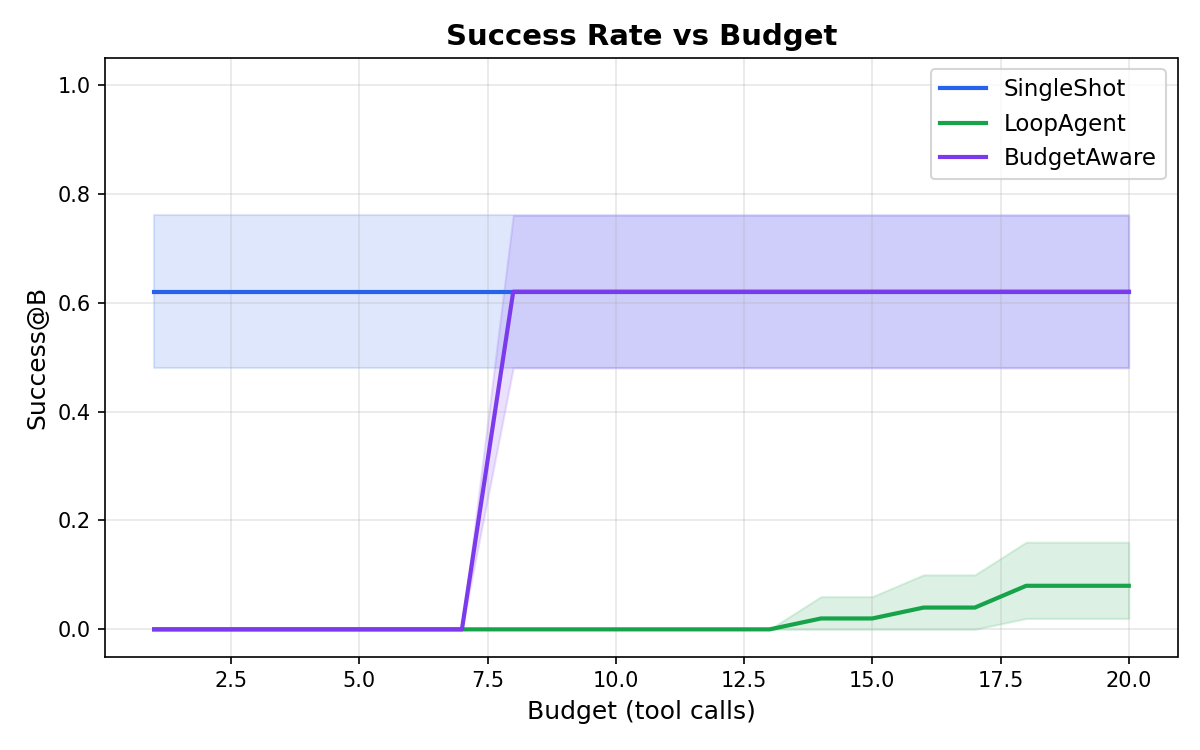
\includegraphics[width=\textwidth]{success_curve.png}
  \end{column}
  \begin{column}{0.48\textwidth}
    \centering
    % Use the knapsack status bars - specify full path to avoid ambiguity
    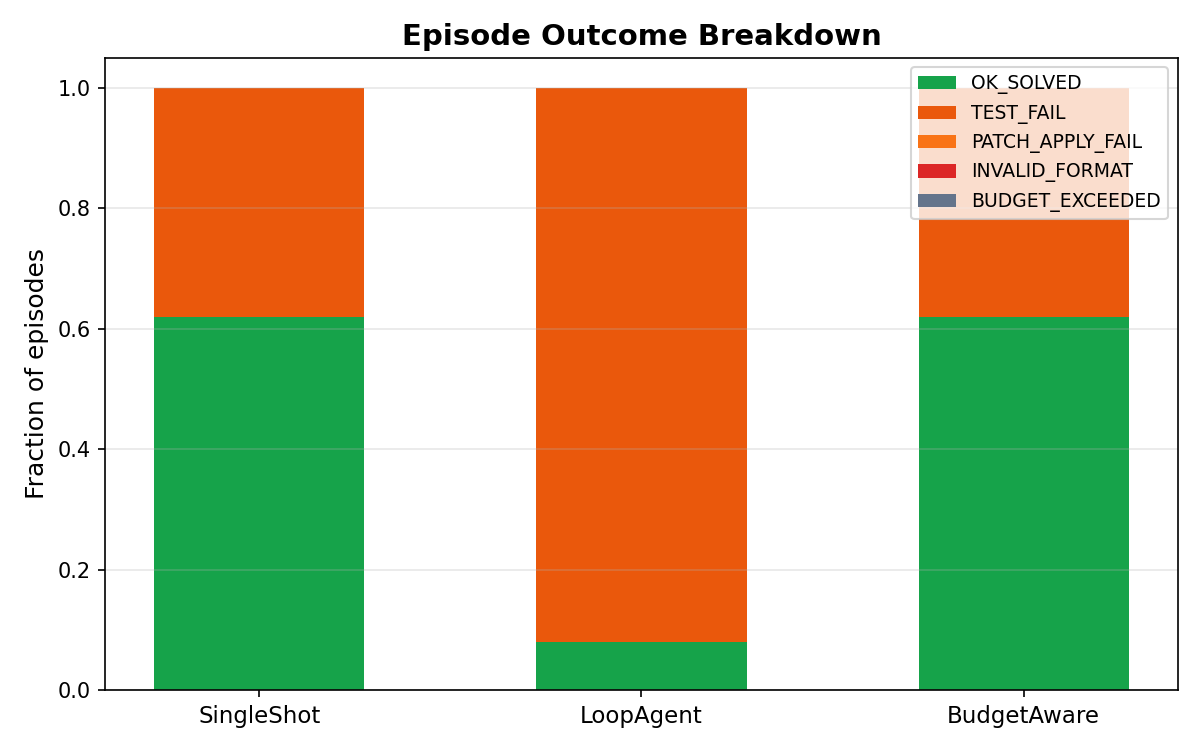
\includegraphics[width=\textwidth]{../results/final/status_bars.png}
  \end{column}
\end{columns}

\vspace{0.2cm}
\begin{beamercolorbox}[wd=\textwidth, rounded=true, sep=4pt]{block body}
  {\footnotesize\textbf{Key finding:} SingleShot and BudgetAware both reach 62\% at all budgets. LoopAgent wastes budget on exploration --- only 8\% at $B{=}20$, all BUDGET\_EXCEEDED at $B{=}5,10$. \textcolor{green}{\textbf{BudgetAware matches SingleShot with 0\% violations.}}}
\end{beamercolorbox}

\end{frame}

% ═══════════════════════════════════════════════════════════════════
% SLIDE 8 — SWE-bench Results
% ═══════════════════════════════════════════════════════════════════
\begin{frame}{SWE-bench Results (Gemini Flash)}

{\small\textcolor{gray}{5 astropy issues $\times$ 3 budgets (10, 20, 30) $\times$ 3 agents~~|~~Docker sandbox + eval images}}

\vspace{0.2cm}
\begin{columns}[c]
  \begin{column}{0.48\textwidth}
    \centering
    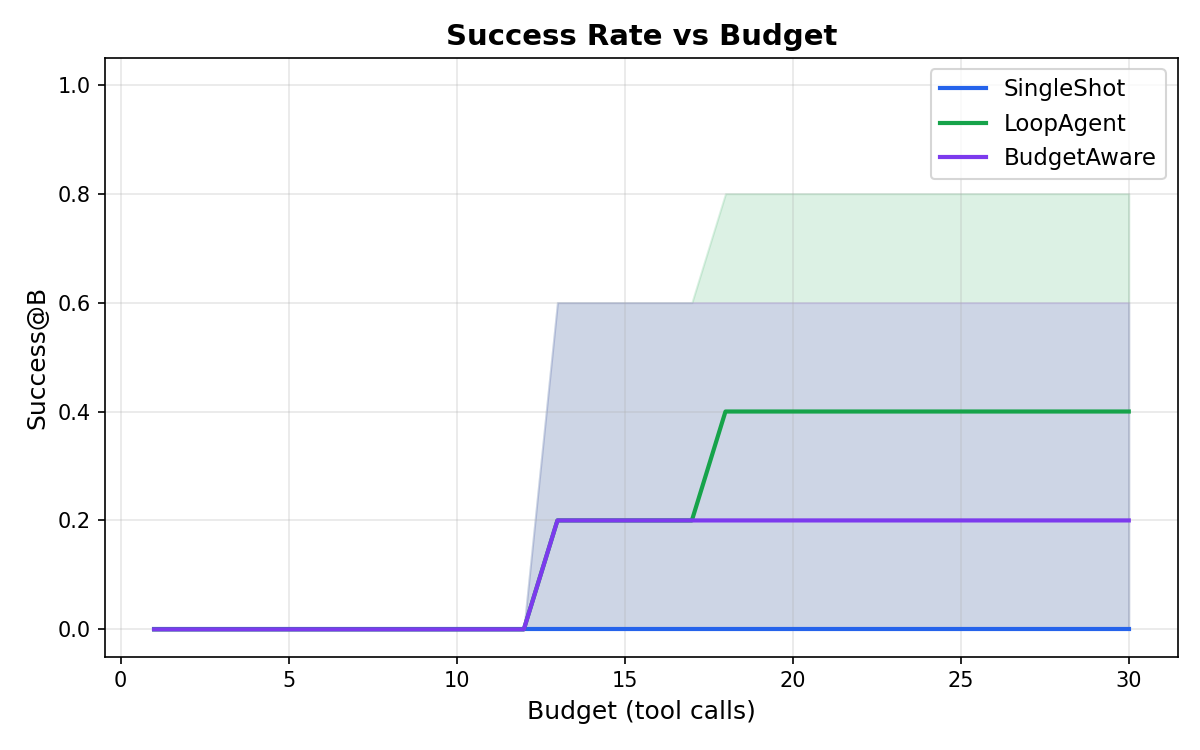
\includegraphics[width=\textwidth]{../results/swe_5issues_flash/success_curve.png}
  \end{column}
  \begin{column}{0.48\textwidth}
    \centering
    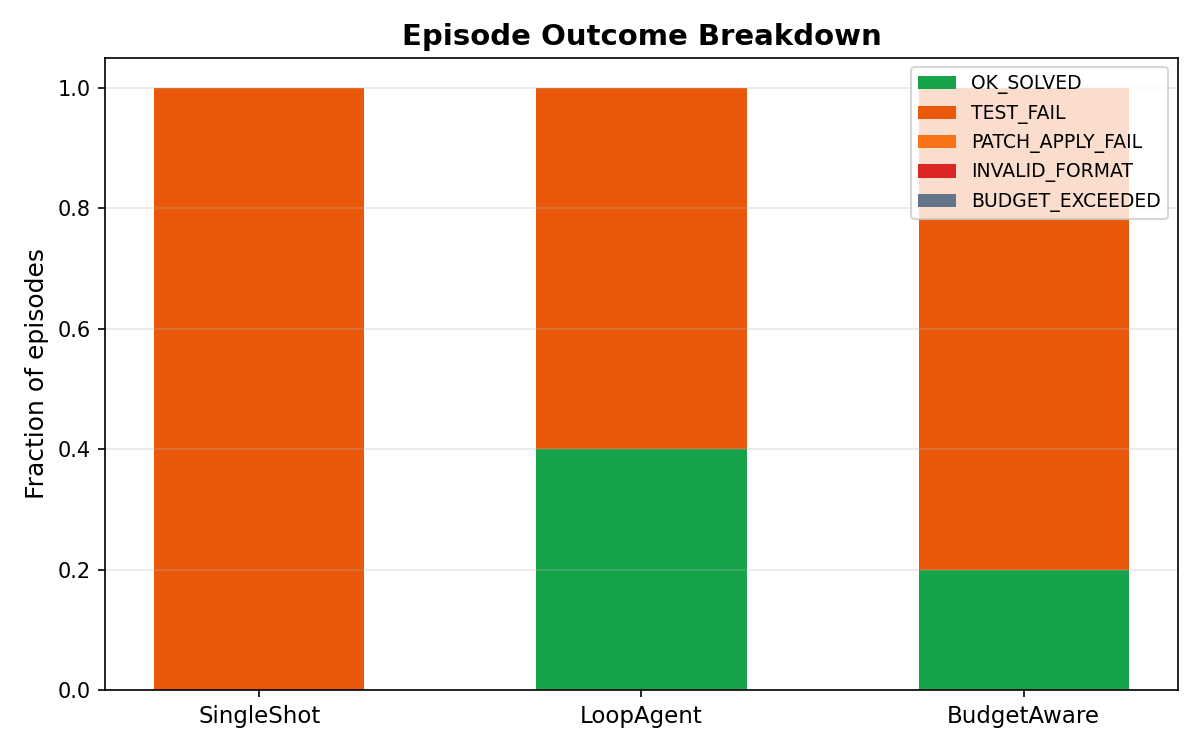
\includegraphics[width=\textwidth]{../results/swe_5issues_flash/status_bars.png}
  \end{column}
\end{columns}

\vspace{0.2cm}
\begin{beamercolorbox}[wd=\textwidth, rounded=true, sep=4pt]{block body}
  {\footnotesize\textbf{Key finding:} LoopAgent reaches 40\% at $B{=}30$ but 0\% at $B{=}10$ (4/5 BUDGET\_EXCEEDED). \textcolor{purple}{\textbf{BudgetAware achieves 20\% at $B{=}10$}} --- the only agent to solve any issue at the lowest budget, with zero violations.}
\end{beamercolorbox}

\end{frame}

% ═══════════════════════════════════════════════════════════════════
% SLIDE 9 — Limitations & Future Work
% ═══════════════════════════════════════════════════════════════════
\begin{frame}{Limitations \& Future Work}

\begin{columns}[T]
  \begin{column}{0.47\textwidth}
    \begin{alertedblock}{Current Limitations}
      {\footnotesize
        \begin{enumerate}
          \item Small SWE-bench sample (5 astropy issues)
          \item Budget = tool calls, not tokens or wall time
          \item Fixed regime thresholds (0.6\,/\,0.3) not tuned
          \item Single LLM backend (Gemini 2.5) tested
          \item No multi-agent architectures compared
        \end{enumerate}
      }
    \end{alertedblock}
  \end{column}
  \begin{column}{0.47\textwidth}
    \begin{exampleblock}{Future Directions}
      {\footnotesize
        \begin{enumerate}
          \item Scale to full SWE-bench Lite (300 issues)
          \item Token-based budget (realistic cost model)
          \item Learned thresholds via Bayesian optimization
          \item Compare Claude, GPT-4, SWE-Agent, etc.
          \item Dynamic budget allocation across subtasks
        \end{enumerate}
      }
    \end{exampleblock}
  \end{column}
\end{columns}

\end{frame}

% ═══════════════════════════════════════════════════════════════════
% SLIDE 10 — Thank You
% ═══════════════════════════════════════════════════════════════════
{
\setbeamercolor{background canvas}{bg=navy}
\begin{frame}[plain]
  \vspace{1.5cm}
  {\Huge\color{white}\textbf{Thank You}}\\[0.3cm]
  {\Large\color{accent!60!white}Questions?}\\[0.8cm]
  {\color{accent!40!white}\rule{3cm}{0.5pt}}\\[0.4cm]
  {\color{white}\footnotesize
    \textbf{Framework:} BudgetRunner + 2 environments + 4 metrics\\[0.1cm]
    \textbf{Agents:} SingleShot, LoopAgent, BudgetAwareAgent\\[0.1cm]
    \textbf{Scale:} 450 Knapsack + 45 SWE-bench episodes\\[0.1cm]
    \textbf{Novelty:} Budget-regime switching with 0\% violation rate
  }\\[0.5cm]
  {\small\color{gray}github.com/Eric-XC/budgetbench}
\end{frame}
}

\end{document}
